\documentclass[12pt]{report}
\usepackage[left=2.5cm, right=2.5cm]{geometry}
\usepackage[utf8]{inputenc}   % For UTF-8 encoding
\usepackage{lipsum}
\usepackage{hyperref}
\usepackage{amsfonts}
\usepackage{listings}
\usepackage{subcaption}
\usepackage{xcolor}
\usepackage{amsthm}
\usepackage{amsmath}
\usepackage{float}
\usepackage{graphicx}
\usepackage{booktabs}
\usepackage{array}
\graphicspath{{imgs/}}
\usepackage{biblatex}
\addbibresource{./sections/referecences.bib}
\usepackage{listings}
\author{Matteo Bordignon, Alessandro Perez, Christian Sassi}
\title{
    
\includegraphics[width=0.7\textwidth]{./imgs/marchio_unitrento_colore_en.png} \\
    \vspace{2 cm}
    \large Advanced Programming of Cryptographic Methods\\
    \vspace{1 cm}
    \small Project Report \\
    \vspace{1.5 cm}
    \huge \textbf{The Rust Unique Secure Talk (T.R.U.S.T)} \\ 
}
\date{\today}

\colorlet{punct}{red!60!black}
\definecolor{background}{HTML}{EEEEEE}
\definecolor{delim}{RGB}{20,105,176}
\colorlet{numb}{magenta!60!black}

\lstdefinelanguage{json}{
    basicstyle=\normalfont\ttfamily,
    numbers=left,
    numberstyle=\scriptsize,
    stepnumber=1,
    numbersep=8pt,
    showstringspaces=false,
    breaklines=true,
    frame=lines,
    backgroundcolor=\color{background},
    literate=
     *{0}{{{\color{numb}0}}}{1}
      {1}{{{\color{numb}1}}}{1}
      {2}{{{\color{numb}2}}}{1}
      {3}{{{\color{numb}3}}}{1}
      {4}{{{\color{numb}4}}}{1}
      {5}{{{\color{numb}5}}}{1}
      {6}{{{\color{numb}6}}}{1}
      {7}{{{\color{numb}7}}}{1}
      {8}{{{\color{numb}8}}}{1}
      {9}{{{\color{numb}9}}}{1}
      {:}{{{\color{punct}{:}}}}{1}
      {,}{{{\color{punct}{,}}}}{1}
      {\{}{{{\color{delim}{\{}}}}{1}
      {\}}{{{\color{delim}{\}}}}}{1}
      {[}{{{\color{delim}{[}}}}{1}
      {]}{{{\color{delim}{]}}}}{1},
}

\begin{document}

\begin{titlepage}
    \maketitle
\end{titlepage}

\tableofcontents
\newpage

\chapter{Introduction}
\label{cha:Inroduction}

This report presents the design, implementation, and evaluation of \textbf{T.R.U.S.T.} (\textbf{T}he \textbf{R}ust \textbf{U}nique \textbf{S}ecure \textbf{T}alk), a terminal user interface (TUI)-based secure chat application developed in Rust. The primary objective of this project was to explore secure communication principles and implement a reliable end-to-end encryption system.

To achieve this purpose we combined different cryptographic primitives to create a key agreement protocol based on \textbf{X3DH} \cite{x3dh} and later encrypt each message with a new key given by the key management scheme: \textbf{Double Ratchet} \cite{DoubleRachet} first introduced by Signal.

The combination of the two gives resilience to both practical and complete leak of the encryption key during the same or different sessions as we will see in later chapters \ref{cha:Security}. More over thanks to the choice of \textbf{Rust} we are sure of not having memory issues or data race conditions, also when a variable is out-of scope we are sure it is set to zero before deleting it.

\section{Organization of the Report}
\label{sec:OrganizationReport}

This document is organized as follows: Introduction \ref{cha:Inroduction} provides an overview of the application’s purpose and core functionalities; Requirements \ref{cha:Requirements} defines both the functional and security requirements; Technical Details \ref{cha:TechnicalDetails} outlines the system’s architecture, the main implementation decisions, and the code structure; Security Considerations \ref{cha:Security} discusses cryptographic measures and potential threats; Known Limitations \ref{cha:Limitations} highlights current constraints and possible improvements; and finally, Instructions for Installation and Execution \ref{cha:Installation} guides readers through setting up and running the application.

\section{Overview of the Protocol}
\label{sec:OverviewProtocol}

The first step to achieve end-to-end encryption is to have a secure method of establishing a shared secrete. There exists many algorithms mainly based on public key cryptography, we decided to implement \textbf{X3DH}, both for its security derived by the Diffie-Hellman algorithm and the use of signatures to prevent miss-bindings compared to the classical implementation of Diffie-Hellman.

\subsection {Extended Triple Diffie-Hellman}
\label{subsec:ExtendedTripleDiffieHellman}

X3DH establishes a shared secret key between two parties who mutually authenticate each other based on public keys. X3DH provides forward secrecy and cryptographic deniability.

This choice was also due to the fact that X3DH is designed for asynchronous settings where one user (“Bob”) is offline but has published some information to a server. Another user (“Alice”) wants to use that information to send encrypted data to Bob, and also establish a shared secret key for future communication.

Before exchanging keys with other users we first need to establish a secure connection between the user and the server so that the server can distribute the correct keys to whoever asks for them. This is done using X3DH between each user and the server we know that this process is secure because the public key of the server is hard-coded and a simple hash of the program ensures integrity.

Once a shared key is established the user can request for any key bundle containing all the necessary keys to start a chat with another user. Now the user can start the establishment of a shared secrete with another user passing through the server. After the shared key is established the two parties will use the Double Ratchet to send and receive encrypted messages.

\subsection{Double Ratchet}
\label{subsec:DoubleRachet}

The parties derive new keys for every message using \textbf{Double Ratchet}, so that earlier keys cannot be calculated from later ones. The parties also send Diffie-Hellman public values attached to their messages. The results of Diffie-Hellman calculations are mixed into the derived keys so that later keys cannot be calculated from earlier ones. These properties give some protection to earlier or later encrypted messages in case of a compromise of a party’s keys.

Now that keys are derived we can send each of the messages encrypted using AES-GCM, an AEAD algorithm, which gives both CCA security and CI. Thanks to all of these algorithms we can have end-to-end encryption and ensure both confidentiality and integrity.


\chapter{Requirements}
\label{cha:Requirements}

\textbf{TRUST} needs to follow a list of both \textbf{functional} requirements and \textbf{security} requirements, these properties are non negotiables, we implemented the application using these requirements as guidelines that helped us in choosing algorithms.

\section{Functional Requirements}
\label{sec:FunRequirements}

This section defines the functional requirements of the system, outlining the core features and expected behaviors necessary for its operation. For this project we can split them further into two sub sets \textbf{server functional requirements} and \textbf{client functional requirements}.

\subsection{Server Functional Requirements}
\label{subsec:ServerFunctionalRequirements}

The server must fulfill the following functional requirements:
\begin{itemize}
    \item \textbf{Manage user registration}
    \item \textbf{Distribute public keys of registered users}
    \item \textbf{Relay encrypted messages to their intended recipients}
\end{itemize}
The server cannot access the content of user messages; it can only identify the sender and recipient.

\subsubsection{Client Functional Requirements}
\label{ClientFunctionalRequirements}

The client application, on the other hand, must meet the following requirements:\begin{itemize}
    \item \textbf{Offer a user-friendly TUI}
    \item \textbf{Allow users to register in the system}
    \item \textbf{Enable users to add others to their contact list}
    \item \textbf{Support message exchange between users}
\end{itemize}
This set of requirements should be enough to have a functional chat application, by adding the \textbf{security requirements} the application will also have: security of data in transit with end-to-end-encryption (E2EE).

\section{Security Requirements}
\label{sec:SecRequirements}

In addition to the functional requirements, we have established the following security requirements:
\begin{itemize}
    \item \textbf{Server Authentication}: Clients must be able to verify the authenticity of the server.
    \item \textbf{Client-Server Confidentiality}: Clients must be able to establish a shared secret with the server.
    \item \textbf{End-to-End Confidentiality}: Clients must be able to establish a shared secret with other clients.
    \item \textbf{End-to-End Integrity}: Clients must use shared secrets to encrypt, decrypt, and verify the integrity of messages exchanged with both the server and other clients.
    \item \textbf{Forward Secrecy}: The compromise of a key must not affect the confidentiality of data exchanged previously.
    \item\textbf{Self Healing (Post Compromise Security)}: even if an adversary temporarily compromises a user's device and obtains current session keys, future messages will remain secure as long as the device regains control and resumes proper ratcheting.
\end{itemize}


\chapter{Technical Details}
\label{cha:TechnicalDetails}

This section provides an in-depth overview of the architecture, implementation, and key components of TRUST. It covers the cryptographic protocols used, system architecture, core libraries, and design decisions that ensure security and usability.

The application is built using Rust’s asynchronous runtime (\texttt{tokio}) and the  framework for networking is \texttt{tokio-tungstenite}, while the user interface is implemented with \texttt{ratatui}. X3DH and Double Ratchet were implemented using primitives provided by the \texttt{dalek-cryptography} library, and AES-GCM using primitives provided by the \texttt{aes\_gcm} library, ensuring end-to-end encryption for user messages.

% TODO bisogna aggiunere la parte di Double Ratchet

\section{Architecture}
\label{sec:Architecture}

The application follows a client-server architecture with some modifications to enhance flexibility. By leveraging \textbf{WebSockets}, which provide bidirectional TCP communication, both the client and server can initiate requests. This approach simplifies development by enabling real-time message exchange without requiring traditional request-response cycles, making the system more efficient and responsive.


\subsection{Architecture overview}
\label{subsec:ArchitectureOverview}
From Server-side, incoming connections from clients are handled leveraging different threads, each responsible for managing a specific client connection.
Upon start up, the server call the \texttt{listen} method which is responsible for accepting incoming connections and spawning a new thread, named \texttt{acceptor}, for each connection. Each thread is responsible for handling the communication with a specific client, allowing the server to manage multiple clients simultaneously. The \texttt{acceptor} thread is responsible for initializing and managing the connection, to doing so, it spaws two additional threads, named \texttt{task\_receiver} and \texttt{task\_sender}. The \texttt{task\_receiver} thread is responsible for listening for incoming requests from the client and send responses back, while the \texttt{task\_sender} thread is responsible for forwarding messages to the client (see fig. \ref{fig:architecture-overview}).
The client, on the other hand, is designed to be a terminal-based user interface (TUI) application that interacts with the server. It consists of a main process that manages the user interface and sends requests to the server, a separate thread for listening to incoming responses or messages and forwarding them to the TUI, ultimetly the TUI levarages on a \texttt{tokio} task that listens for incoming messages on a \texttt{mpsc channel} and invokes the appropriate handler to process the message and render it in the user interface (see fig. \ref{fig:client-architecture-overview}).\\

To better understand the application's functionality, we outline four key scenarios that define its core operations:

\begin{enumerate}
    \item \textbf{Establishment of a Secure Connection}: The client and server perform a handshake to initiate a secure, encrypted communication channel.
    \item \textbf{User Registration}: New users send their public keys and register with the server while ensuring their identity remains protected.
    \item \textbf{Adding a Friend}: Users exchange public keys and establish a secure communication channel for encrypted messaging.
    \item \textbf{Sending Messages}: Messages are encrypted, transmitted over WebSockets, and decrypted on the recipient’s side, ensuring end-to-end security.
\end{enumerate}

Each of these steps plays a crucial role in maintaining the privacy and integrity of user interactions. The following sections describe these scenarios in detail.

\subsection{Establishment of a Secure Connection}
\label{subsec:EstablishmentOfASecureConnection}

The secure connection process begins with a standard \textbf{WebSocket handshake} (Figure \ref{fig:websocket-handshake}) between the client and server. Once the bidirectional channel is established, the client transmits its \textbf{Pre-Key Bundle}, which the server processes to:

\begin{itemize}
    \item Derive the shared key used to encrypt communications.
    \item Generate the \textbf{Server Initial Message (SIM)}, which is then sent back to the client.
\end{itemize}

\begin{figure}[!ht]
    \centering
    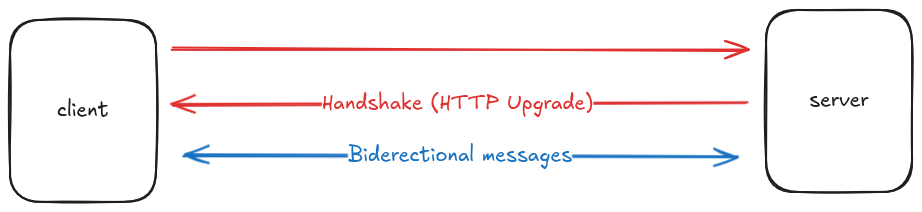
\includegraphics[width=0.8\linewidth]{imgs/Websocket.png}
    \caption{WebSocket Handshake}
    \label{fig:websocket-handshake}
\end{figure}

Upon receiving the SIM, the client verifies the server’s identity by comparing the known \textbf{server public identity key} with the one provided in the message. This prevents \textbf{Man-in-the-Middle (MitM) attacks}. If authentication is successful, the client processes the SIM and derives the shared key. From this point forward, all communication between the client and server will be encrypted.

\begin{figure}[!ht]
    \centering
    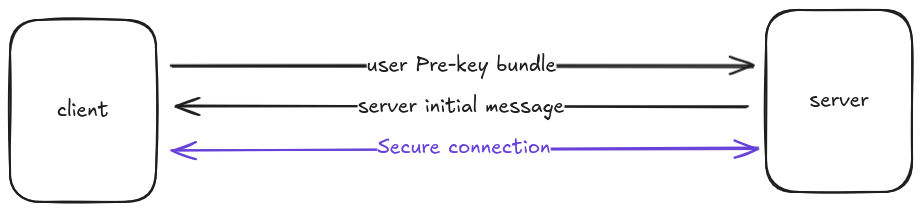
\includegraphics[width=0.8\linewidth]{imgs/secure-connection.png}
    \caption{Secure connection establishment}
    \label{fig:secure-connection}
\end{figure}

\subsection{User Registration}
\label{subsec:UserRegistration}

Once a secure connection with the server is established, the user can register by choosing a \textbf{username} and sending a \textbf{registration request} to the server. The server then verifies whether the chosen username is unique.

\begin{itemize}
    \item If the username is \textbf{available}, the server sends a \textbf{confirmation response} to the client.
    \item If the username is \textbf{already taken}, the server responds with a \texttt{"Conflict"} status code and the message \texttt{"User Already Exists"}, prompting the user to choose a different username.
\end{itemize}

\begin{lstlisting}[language=json, caption= Example of a Registration request]
{
    "action":"register",
    "username":"xyz",
    "bundle:"dGhpcyBpcyB0aGUgdXNlciBwcmVrZXkgYnVuZGxGluIGJ2U2NA=="
}
\end{lstlisting}

\subsection{Adding a Friend}
\label{subsec:AddingAFriend}

Once the user is registered in the system, they can add a new friend by submitting a \textbf{get user pre-key bundle request} to the server, specifying the username of the desired contact. The server then checks whether the requested user is registered in the application.

\begin{itemize}
    \item If the user \textbf{exists}, the server responds with the requested user's \textbf{Pre-Key Bundle}.
    \item If the user \textbf{is not found}, the server returns a \texttt{"UserNotFound"} error response with \texttt{status code 404}.
\end{itemize}

\subsection{Sending Messages}
\label{subsec:SendingMessages}

% TODO bisogna aggiunere la parte di Double Ratchet

Upon receiving the requested user's \textbf{Pre-Key Bundle}, the user derives the \textbf{shared key} and generates the \textbf{initial message}. The user then sends a \texttt{send\_message} request to the recipient, embedding the initial message in the \texttt{"text"} field. The request follows the JSON format below:

\begin{lstlisting}[language=json, caption={Initial Message Request Format}]
{
  "action": "send_message",
  "msg_type": "initial_message",
  "to": "alice",
  "from": "bob",
  "text": "dGhpcyBpcyB0aGXNlciBpbml0aWFsIG1lc3NhZ2UgaW4gYmFzZTY0",
  "timestamp": "2025-02-06T14:21:21+00:00"
}
\end{lstlisting}

The user who will receive the initial message will derive the shared key and then add the sender as a contact in their contacts list.

\section{Implementation}
\label{sec:Implementation}

This section will provide a comprehensive explanation of the implementation of each key component of the application. Each aspect of the application, from the underlying security mechanisms to the user-facing interface, is discussed in detail to give a clear understanding of the technical choices and how they come together to ensure a seamless and secure user experience.

\subsection{Key Generation for X3DH}
\label{subsec:KeyGeneration}

The function responsible for generating \textbf{Pre-Key Bundles} is \texttt{generate\_prekey\_bundle()}. This function creates the \textbf{Private Identity Key}, \textbf{Private Signed Pre-Key}, and their corresponding \textbf{Public Keys}. Additionally, it returns the \textbf{Pre-Key Bundle} along with the \textbf{private keys} required for secure communication.

To prevent \textbf{replay attacks}, \textbf{One-Time Pre-Keys (OTPKs)} are incorporated into the key generation process. For this purpose, a specialized function, \\ \texttt{generate\_prekey\_bundle\_with\_otpk()}, is introduced. This function takes as input the number of \textbf{one-time pre-keys} to generate and returns a tuple containing:
\begin{itemize}
    \item The \textbf{Pre-Key Bundle},
    \item The \textbf{Private Identity Key},
    \item The \textbf{Private Signed Pre-Key},
    \item A vector of \textbf{private One-Time Pre-Keys}.
\end{itemize}

This approach ensures that each session can maintain \textbf{forward secrecy} while mitigating potential security risks such as \textbf{key reuse and replay attacks}.

\subsection{Pre-Key Bundle Processing}
\label{subsec:Pre-KeyBundleProcessing}

The function responsible for processing \textbf{Pre-Key Bundles} is \texttt{process\_prekey\_bundle()}, which takes as input the received bundle and the receiver's \textbf{Private Identity Key}.

The function first verifies the signature contained in the bundle to ensure its authenticity. After validation, it performs the \textbf{X3DH (Extended Triple Diffie-Hellman) key agreement protocol} to derive the shared secret. This is done by passing the secret obtained from the three Diffie-Hellman exchanges through a \textbf{Key Derivation Function (KDF)} to generate the final 32-byte shared key.  

Once the shared key is established, an \textbf{Initial Message (IM)} is generated, containing the following components:  

\begin{itemize}  
    \item The receiver's \textbf{Public Identity Key};  
    \item The receiver's \textbf{Public Ephemeral Key};  
    \item The sender's \textbf{Public Signed Pre-Key hash} (extracted from the bundle);  
    \item The sender's \textbf{Public One-Time Pre-Key (OTPK) hash};  
    \item \textbf{Associated Data}, which includes the Public Identity Keys of both the sender and receiver.  
\end{itemize}  

The function then returns the shared key and the initial message.

\subsection{Initial Message Processing}
\label{subsec:InitialMessageProcessing}

The functions responsible for processing the \textbf{Initial Message} are respectively \\ \texttt{process\_server\_initial\_message()} and \texttt{process\_initial\_message()}. These two functions are equivalent, except that the former additionally verifies whether the \textbf{Server's Public Identity Key} provided as input matches the one included in the Initial Message.  

Both functions take as input the received Initial Message, the receiver's \textbf{Private Identity Key}, \textbf{Private Signed Key}, and \textbf{Private One-Time Pre-Key (OTPK)}. They compute the three Diffie-Hellman (3DH) secrets and pass the resulting value through a \textbf{Key Derivation Function (KDF)} to derive the 32-byte shared key. Finally, they return the computed shared key.  

\subsection{AES Encryption}
\label{subsec:AESEncryption}

The function responsible for AES encryption is \texttt{encrypt()}. This function takes as input the encryption key, the data to be encrypted, and the \textbf{Associated Data (AD)}.

First, it generates a nonce using the Cryptographically Secure Pseudo Random Number Generator (CSPRNG) provided by the \texttt{rand} crate in Rust (OsRng). Then, it constructs the payload and performs AES-GCM encryption. Finally, it concatenates the nonce, the associated data, and the ciphertext before returning the result as a \textbf{Base64-encoded string}.

\subsection{AES Decryption}
\label{subsec:AESDecryption}

The function responsible for AES decryption is \texttt{decrypt()}. It takes as input the decryption key, the cipher text to be decrypted, and the \textbf{Associated Data (AD)} and the \textbf{Nonce}.

This function checks for integrity and then performs the inverse operation of the encryption process if the message has not been tampered with. Finally, it returns the decrypted data as a \textbf{byte vector}.


\subsection{Server}
\label{subsec:Server}
The server implementation is built on an asynchronous runtime provided by the \texttt{tokio} library in Rust. This library enables the server to perform non-blocking asynchronous operations, improving both flexibility and performance.  

Each new connection is handled by a separate Tokio task, allowing the server to efficiently manage multiple concurrent connections. For each \textbf{Connection task}, two additional Tokio tasks are generated:

\begin{itemize}
    \item the first task (\texttt{task\_receiver}) continuously listen for incoming requests;
    \item the second task (\texttt{task\_sender}) forwards messages to the client;
\end{itemize}

\subsubsection{Task Receiver}
\label{subsec:TaskReceiver}

This task continuously listens for incoming requests on the WebSocket connection from the client. It exposes four API endpoints:

\begin{itemize}
    \item \texttt{establish\_connection}: Used to establish a secure connection between the client and the server. This API endpoint is handled by the function \\
    \texttt{handle\_establish\_connection()}, which first verifies whether the Pre-Key bundle is correctly formatted. If the verification is successful, the function calls  \\
    \texttt{process\_key\_bundle()} to generate the shared secret; otherwise, it returns an error. Once the shared secret is derived, it is stored in a shared variable called \texttt{session}, allowing both tasks to access it. This endpoint is only accessible if no shared secret exists, meaning that a secure connection has not yet been established.

    \item \texttt{register}: Accessible once the secure connection is established, allowing the client to register within the application. This API endpoint is handled by the function \texttt{handle\_registration\_request()}, which first performs the necessary username validation (ensuring it is alphanumeric and not already in use). It then verifies whether the Pre-Key bundle is well-formed. If all checks pass, the user is registered in the system and it sends back a confirmation response.

    \item \texttt{get\_user\_bundle}: Accessible after the secure connection is established, enabling the client to retrieve a user's key bundle. This API endpoint is handled by the function \texttt{handle\_get\_bundle\_request()}, which verifies whether the requested user is registered in the system. If the user exists, the function generates a response containing the corresponding key bundle; otherwise, it returns a \texttt{User Not Found} error.

    \item \texttt{send\_message}: Available once the secure connection is established, allowing the client to exchange messages with other users. This API endpoint is handled directly by the task. It first checks whether the recipient is registered (and thus connected) to the system. If the recipient is online, the task forwards the message to the recipient's sender task, which then delivers it to the recipient's client.
\end{itemize}

All API requests received after the secure connection is established are decrypted upon arrival, and all responses are encrypted before being sent to the client. 

\subsubsection{Task Sender}
\label{subsec:TaskSender}

The Task Sender is responsible for message forwarding. It continuously listens on a \texttt{mpsc channel} for incoming messages. Upon receiving a message, it encrypts the content using the session key shared between the recipient client and the server, ensuring secure communication. Once the message is encrypted, it forwards the encrypted message to the recipient.

The content of messages is encrypted using the shared key between the two clients. The \texttt{send\_message} request undergoes two layers of encryption: first, the message text is encrypted with the shared key between the clients, and then the entire request is encrypted using the shared key between the client and the server, ensuring end-to-end security.

%put image here
\begin{figure}
  \centering
  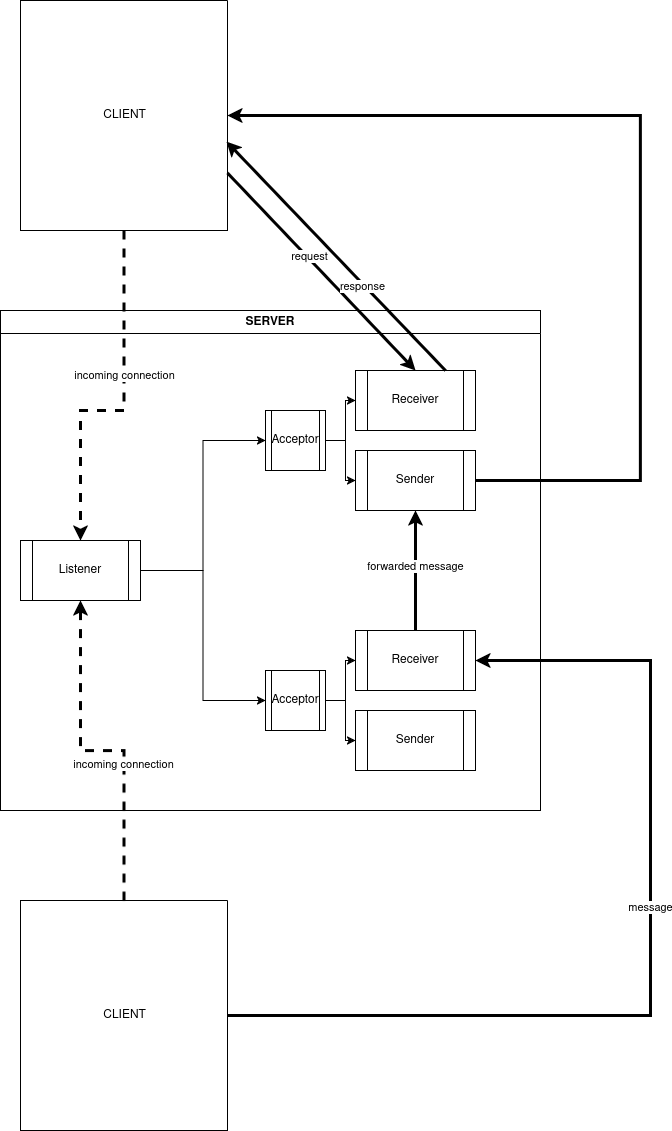
\includegraphics[width=0.8\linewidth]{imgs/server-arch.png}
  \caption{Server Architecture Overview}
  \label{fig:architecture-overview}
\end{figure}



\begin{figure}
  \centering
  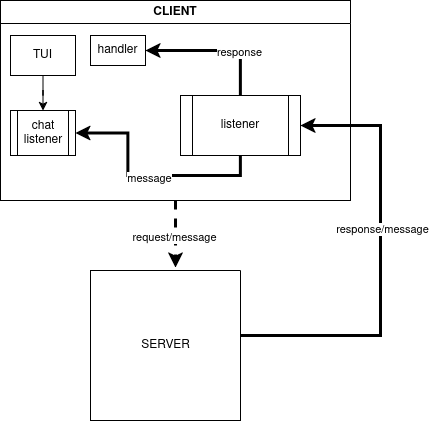
\includegraphics[width=0.8\linewidth]{imgs/client-arch.png}
  \caption{Client Architecture Overview}
  \label{fig:client-architecture-overview}
\end{figure}

\subsection{Client \& TUI}
\label{subsec:ClientTUI}

The client backend also utilizes \texttt{tokio} for asynchronous runtime. When a new client is created (i.e., when the TUI program is started), it attempts to establish a secure connection with the server. If successful, it spawns a Tokio listener task, which continuously listens for incoming responses or new messages.  

To manage the correlation between requests and responses, we introduced a struct called \texttt{RequestWrapper}. This struct contains two fields: \texttt{request\_uuid}, which uniquely identifies the request, and \texttt{body}, which holds the actual request to be sent to the server. When the server responds, it includes the same \texttt{request\_uuid} in the \texttt{ResponseWrapper}, allowing the client to match each response to its corresponding request.  

Chat messages, on the other hand, are handled as regular \texttt{send\_message} requests. When the client receives a message, it forwards it to a task running in the TUI binary, which listens for incoming messages on a \texttt{mpsc channel}. This task then invokes the appropriate handler to process the message and render it in the user interface.
\newpage
\section{Code Structure}
\label{sec:CodeStructure}

%TODO la struttura e' cambiata aggiungendo la perte di dr

The codebase is organized into five separate Cargo projects, each serving a distinct purpose:

\begin{itemize}
    \item \textbf{Protocol}: A library that implements the cryptographic protocols used in the system, including X3DH and AES-GCM.
    \item \textbf{Common}: A shared library providing utility functions used by both the client and server.
    \item \textbf{Server}: Contains the server binary along with all necessary utility functions for server-side operations.
    \item \textbf{Client}: A library that facilitates client interactions with the server.
    \item \textbf{Tui}: Includes the TUI application binary, along with all files required for the user interface and front-end logic.
\end{itemize}

\section{Dependencies}
\label{sec:Dependecies}

% TODO non sono sicuro se dr abbia aggiunto altre dependencies ma se si bisogna aggiungerle

The implementation of \textbf{TRUST} application relies on several external Rust crates that provide critical functionalities such as asynchronous networking, cryptographic operations, and terminal user interface (TUI) rendering. All dependencies used in this project are well-known, actively maintained, and considered de facto standards in their respective domains, ensuring reliability, security, and long-term support. Below is an overview of the main dependencies.   

\subsection{Networking and Asynchronous Execution}
\label{subsec:NetworkingAndAsynchronousExecution}

The list of dependencies used for the asynchronous execution is:

\begin{itemize}
  \item \textbf{\texttt{tokio} (1.42.0)}: Provides the asynchronous runtime used throughout the application to handle concurrent tasks efficiently, enabling non-blocking communication between clients and the server.
  \item \textbf{\texttt{tokio-tungstenite} (0.26.1)}: A WebSocket library that integrates with Tokio, allowing real-time, bidirectional communication over WebSockets.
  \item \textbf{\texttt{futures} (0.3.31) \& \texttt{futures-util} (0.3.31)}: Provide abstractions for asynchronous programming, including streams and futures for handling asynchronous events.
  \item \textbf{\texttt{tokio-stream} (0.1.17)}: Enhances stream handling within Tokio-based applications, making it easier to process asynchronous data flows.
\end{itemize}

\subsection{Cryptography and Secure Communication}
\label{subsec:CryptographyAndSecureCommunication}

The list of dependencies used for cryptographic purposes on the other hand is:

\begin{itemize}
  \item \textbf{\texttt{aes} (0.8.4) \& \texttt{aes-gcm} (0.10.3)}: Provide authenticated encryption for securing messages using the AES-GCM encryption scheme.
  \item \textbf{\texttt{rand} (0.8.5)}: A cryptographically secure random number generator, essential for generating nonces securely.
  \item \textbf{\texttt{ed25519-dalek} (2.1.1)}: Implements the Ed25519 signature scheme, ensuring authentication and integrity of messages.
  \item \textbf{\texttt{x25519-dalek} (2.0.1)}: Used for implementing the X3DH key exchange protocol, allowing secure key agreement between clients.
  \item \textbf{\texttt{curve25519-dalek} (4.1.3)}: Provides elliptic curve operations, specifically for Diffie-Hellman key exchange and digital signatures.
  \item \textbf{\texttt{sha2} (0.10.8)}: Implements the SHA-2 family of cryptographic hash functions, ensuring data integrity and secure hashing of credentials.
  \item \textbf{\texttt{hkdf} (0.12.4)}: Implements the HMAC-based Key Derivation Function (HKDF) used to derive cryptographic keys securely.
  \item \textbf{\texttt{zeroize} (1.8.1)}: Ensures that sensitive cryptographic data is securely erased from memory when no longer needed.
\end{itemize}

\subsection{Data Serialization and Parsing}  
\label{subsec:DataSerializatinAndParsin}

The dependencies used for data serialization is:

\begin{itemize}
  \item \textbf{\texttt{serde} (1.0.216) \& \texttt{serde\_json} (1.0.137)}: Used for serializing and deserializing data exchanged between the client and server.
  \item \textbf{\texttt{base64} (0.22.1)}: Handles encoding and decoding of binary data, particularly for securely transmitting encrypted messages.
\end{itemize}

\subsection{Terminal User Interface (TUI)}  
\label{subsed:TerminalUserInterfaceTUI}

For the TUI we chose the following dependencies:

\begin{itemize}
  \item \textbf{\texttt{ratatui} (0.29.0)}: A Rust TUI library used to create the command-line interface for the chat application.
  \item \textbf{\texttt{crossterm} (0.28.1)}: Provides cross-platform support for handling terminal input and output, including event handling and text rendering.
\end{itemize}

\subsection{Utilities}
\label{subsec:Utilities}

Finally some extra packeges chosen for extra utilities are:

\begin{itemize}
  \item \textbf{\texttt{uuid} (1.11.0)}: Used for generating unique request identifiers, allowing the system to match server responses with client requests.
  \item \textbf{\texttt{arrayref} (0.3.9)}: Provides utilities for working with fixed-size arrays, useful in cryptographic operations.
\end{itemize}

These dependencies collectively enable our application to provide secure, efficient, and user-friendly encrypted messaging.  


\chapter{Security Considerations}
\label{cha:Security}

In this chapter we are going to discuss in more details the cryptographic principles that ensure security. Firstly we are going to analyze X3DH and later the double ratchet mechanism. But before starting we need to define some preliminaries used in each of the two algorithms.

\section{Preliminaries}
\label{sec:Preliminaries}

As explained above an application using X3DH must decide on several parameters:

\vspace{0.5cm}
\begin{center}
\begin{tabular}{>{\itshape}l p{10cm}}
\toprule
Name & Definition \\
\midrule
curve & X25519 or X448 \\
hash & A 256 or 512-bit hash function (e.g. SHA-256 or SHA-512) \\
info & An ASCII string identifying the application \\
\bottomrule
\end{tabular}
\end{center}

\vspace{0.5cm}

In our protocol we used \textbf{X25519}, as hash \textbf{SHA}. An application must additionally define an encoding function Encode(PK) to encode an X25519 or X448 public key PK into a byte sequence. Since we decided to implement only one of the two curves there was no need to differentiate between them.

\section{Cryptographic Notation}
\label{sec:Crytpographic Notation}

The used notation in this chapter is:

\begin{itemize}
  \item The concatenation of byte sequences \textbf{X} and \textbf{Y} is $\textbf{X} \| \textbf{Y}$
  \item $\textbf{DH(PK1,PK2)}$ represents a byte sequence which is the shared secret output from an Elliptic Curve Diffie-Hellman function involving the key pairs represented by public keys $PK1$ and $PK2$. The Elliptic Curve Diffie-Hellman function will be the $X25519$.
  \item $\textbf{Sig(PK,M)}$ represents a byte sequence that is an \textbf{XEdDSA} signature on the byte sequence $M$ and verifies with public key $PK$, and which was created by signing $M$ with $PK$'s corresponding private key.
  \item \textbf{KDF(KM)} represents 32 bytes of output from the $HKDF$ algorithm with inputs:
  \begin{itemize}
    \item $HKDF$ $input$ $key$ $material = F \| KM$, where $KM$ is an input byte sequence containing secret key material, and $F$ is a byte sequence containing $32$ $0xFF$. $F$ is used for cryptographic domain separation with $XEdDSA$.
    \item $HKDF$ $salt =$ a zero-filled byte sequence with length equal to the $hash$ output length.
    \item $HKDF$ $info =$ the $info$ parameter.
  \end{itemize}
\end{itemize}

\section{Roles}
\label{sec:Roles}

The X3DH protocol involves theree parties: \textbf{Alice, Bob} and a \textbf{server}.

\begin{itemize}
  \item \textbf{Alice} wants to send to Bob some initial data using encryption, and also establish a shared secret key.
  \item \textbf{Bob} wants to allow parties like Alice to establish a shared key with him and send encrypted data. However, Bob might be offline when Alice attempts to do this. To enable this, Bob has a relationship with some server.
  \item \textbf{The server} can store messages from Alice to Bob which Bob can later retrieve. The server also lets Bob publish some data which the server will provide to parties like Alice.
\end{itemize}

\section{Keys}
\label{sec:Keys}

X3DH used the following elliptic curve keys:

\begin{center}
\begin{tabular}{>{\itshape}l l}
\toprule
Name & Definition \\
\midrule
$IK_A$ & Alice’s identity key \\
$EK_A$ & Alice’s ephemeral key \\
$IK_B$ & Bob’s identity key \\
$SPK_B$ & Bob’s signed prekey \\
$OPK_B$ & Bob’s one-time prekey \\
\bottomrule
\end{tabular}
\end{center}

All public keys have a corresponding private key, but to simplify description we will focus on the public keys. Each party has a long-term identity public key ($IK_A$ for Alice, $IK_B$ for Bob). Bob also has a signed prekey $SPK_B$, which he will change periodically, and a set of one-time prekeys $OPK_B$, which are each used in a single X3DH protocol run. During each protocol run, Alice generates a new ephemeral key pair with pubic key $EK_A$. After a successful protocol run Alice and Bob will share a 32-byte secret key $SK$ that later will be used a root key for the double ratchet.

\section{The X3DH protocol}
\label{sec:TheX3DHProtocol}

X3DH has three pahses:

\begin{enumerate}
  \item Bob publishes his identity key and prekeys to a server.
  \item Alice fetches a prekey bundle from the server, and uses it to send an initial message to Bob.
  \item Bob receives and processes Alice's initial message.
\end{enumerate}

\section{Publishing Keys}
\label{sec:PublishingKeys}

Bob publishes a set of elliptic curve public keys to the server, containing:

\begin{itemize}
  \item Bob's identity key $IK_B$
  \item Bob's signed prekey $SPK_B$
  \item Bob's prekey signature $Sig(IK_B, Encode(SPK_B))$
  \item A set of Bob's one-time prekeys $(OPK_B^1, OPK_B^2, OPK_B^3, ...)$
\end{itemize}

Bob only needs to upload his identity key to the server once. However, Bob may upload new one-time prekeys at other times. Bob will also upload a new signed prekey and prekey signature at some interval. The new signed prekey and prekey signature will replace the previous values.

\section{Sending the Initial Message}
\label{sec:SendingTheInitialMessage}

To perform an X3DH key agreement with Bob, Alice contacts the server and fetches a prekey bundle containing the following values:
  
\begin{itemize}
  \item Bob's identity key $IK_B$
  \item Bob's signed prekey $SPK_B$
  \item Bob's prekey signature $Sig(IK_B, Encode(SPK_B))$
  \item Bob's one-time prekey $OPK_B$
\end{itemize}

The serve provides one of Bob's one-time prekeys, and then delete it. Alice verifies the prekey signature and aborts the protocol if verification fails. Alice then generates an ephemeral key pair with public key $EK_A$.

Alice calculates:

\begin{itemize}
  \item $DH1 = DH(IK_A, SPK_B)$
  \item $DH2 = DH(EK_A, IK_B)$
  \item $DH3 = DH(EK_A, SPK_B)$
  \item $DH4 = DH(EK_A, OPK_B)$
  \item $SK = KDF(DH1 \| DH2 \| DH3 \| DH4)$
\end{itemize}

Note that $DH1$ and $DH2$ provide mutual authentication, while $DH3$ and $DH4$ provide forward secrecy. After calculating $SK$, Alice deletes her ephemeral private key and the $DH$ outputs. Alice then calculates an AD byte sequence that contains identity information for both parties: $AD = Encode(IK_A) \| Encode(IK_B)$.

Alice then sends Bob an initial message containing:

\begin{itemize}
  \item Alice's identity key $IK_A$
  \item Alice's ephemeral key $EK_A$
  \item Identifiers starting which of Bob's prekeys Alice used
  \item An initial ciphertext encrypted with AES-GCM using AD as associated data.
\end{itemize}

This first ciphertext is used both as the first message within the double ratchet, and as part of Alice's X3DH initial message.

\section{Receiving the Initial Message}
\label{sec:ReceivingTheInitialMessage}

Upon receiving Alice's initial message, Bob retrieves Alice's identity key and ephemeral key from the message. Bob also loads his identity private key, and the private key(s) corresponding to whichever signed prekey and one-time prekey Alice used.

Using these keys, Bob repeats the DH and $KDF$ calculations from the previous section to derive SK, and then deletes the DH values. Bob then constructs the AD byte sequence using $IK_A$ and $IK_B$, as described in the previous section. Finally, Bob attempts to decrypt the initial ciphertext using SK and AD. If the initial ciphertext fails to decrypt, then Bob aborts the protocol and deletes SK. If the initial ciphertext decrypts successfully the protocol is complete for Bob. Bob deletes any one-time prekey private key that was used, for forward secrecy.

\section{Double Ratchet}
\label{sec:DoubleRatchet}

\subsection{KDF Chains}
\label{subsec:KDF Chains}
We define a \textbf{KDF} as a cryptographic function that takes a secret and random \textbf{KDF key} and some input data and returns output data. The output data is indistinguishable from random provided the key isn't known. If the key is not secret and random, the KDF should still provide a secure cryptographic hash of its key and input data. The HMAC and HKDF construction, we chose has a secure hash algorithm, as it meets the KDF definition.

The term \textbf{KDF chain} is used when some of the output from KDF is used as an \textbf{output key} and some is used to replace the KDF key, which can then be used with another input.

\begin{figure}[ht!]
  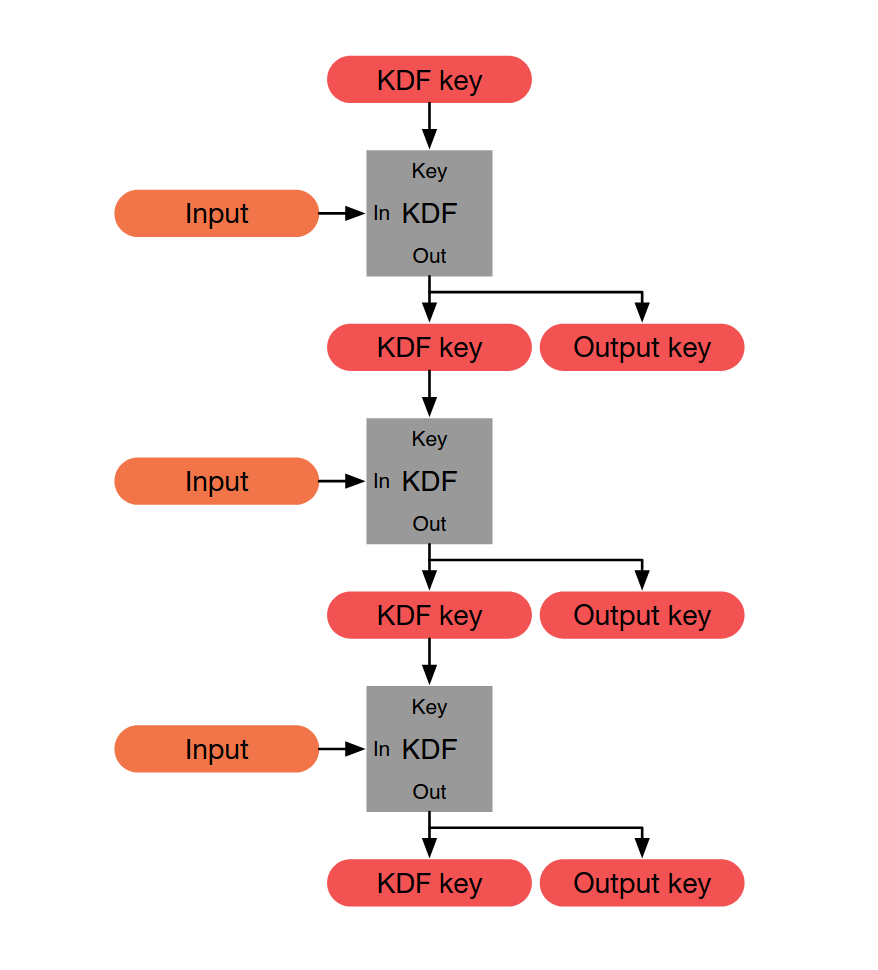
\includegraphics[scale=0.3]{KDF_Chain.png}
  \centering
\end{figure}

A KDF chain has the following properties:

\begin{itemize}
  \item \textbf{Resilience:} The output keys appear random to an adversary without knowledge of the KDF keys. This is true even if the adversary can control the KDF inputs.
  \item \textbf{Forward security:} Output keys from the past appear random to an adversary who learns the KDF key at some point in time.
  \item \textbf{Break-in recovery:} Future output keys appear random to an adversary who learns the KDF key at some point in time, provided that future inputs have added sufficient entropy.
\end{itemize}

In a \textbf{Double ratchet session} between Alice and Bob each party stores a KDF key for three chains: a \textbf{root chain}, a \textbf{sending chain}, and a \textbf{receiving chain}.

As Alice and Bob exchange messages they also exchange new Diffie-Hellman public keys, and the Diffie-Hellman output secretes become the inputs to the root chain. The output keys from the root chain become new KDF keys for the sending and receiving chains. This is called the \textbf{Diffie-Hellman ratchet}.

The sending and receiving chains advanced as each message is sent and received. Their output keys are used to encrypt and decrypt messages. This is called the \textbf{symmetric-key ratchet}.

\subsection{Symmetric-key ratchet}
\label{subsec: Symmetric-keyRatchet}

Every message sent or received is encrypted with a unique \textbf{message key}. The message keys are output keys from the sending and receiving KDF chains. The KDF keys for these chains will be called \textbf{chain keys}.

The KDF inputs for the sending and receiving chains are constant, so these chains don't provide break-in recovery. The sending and receiving chains just ensure that each message is encrypted with a unique key that can be deleted after encryption or decryption. Calculating the next chain key and message key from a given chain key is a single \textbf{ratchet step} in the \textbf{symmetric-key ratchet}.

Since message keys are not used to derive any other keys, message keys may be stored without affecting the security of other message keys. This property is useful for handling lost or out of order messages.

\subsection{Diffie-Hellman ratchet}
\label{subsec:Diffie-HellmanRatchet}

If an attacker steals on party's sending and receiving chain keys, the attacker can compute and decrypt all future messages. To prevent this, the Double Ratchet combines the symmetric-key ratchet with a \textbf{DH ratchet} which updates chain keys based on Diffie-Hellman outputs.

To implement the DH ratchet, each party generates a DH key pair which becomes their current \textbf{ratchet key pair}. Every message from either party begins with a header which contains the sender's current ratchet public key. When a new ratchet public key is received from the remote party, a \textbf{DH ratchet step} is performed which replaces the local party's current ratchet key pair with a new key pair.

This results in a "ping-pong" behavior as the parties take turns replacing ratchet key pairs. An eavesdropper who briefly compromises one of the parties might learn that value of a current ratchet private key, but that private key will eventually be replaced with an uncompromised one. A that point, the Diffie-Hellman calculation between ratchet key pairs will define a DH output unknown to the attacker.

\newpage

\begin{figure}[ht!]
  \centering
  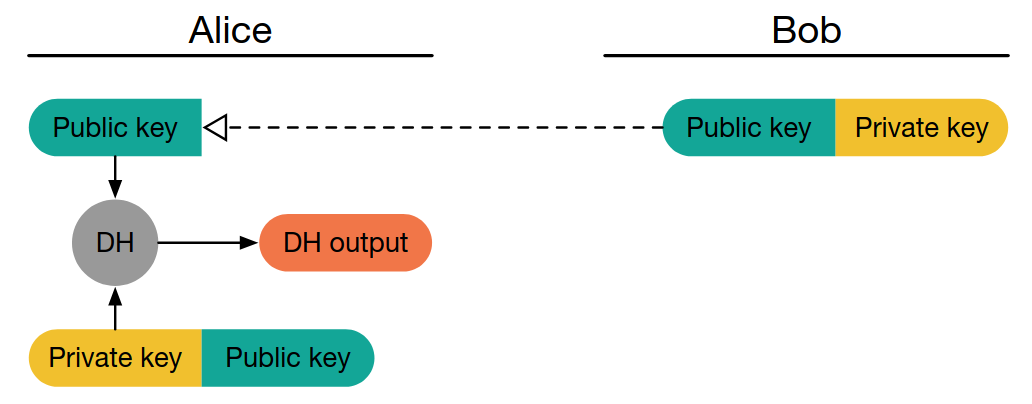
\includegraphics[scale=0.25]{dr1.png}
  \caption{}
  \label{fig:dr1}
\end{figure}

Alice is initialized with Bob's ratchet public key. Alice's ratchet public key isn't yet known to Bob. A part of initialization Alice perform a DH calculation between her ratchet private key and Bob's ratchet public key as shown in figure \ref{fig:dr1}

\begin{figure}[ht!]
  \centering
  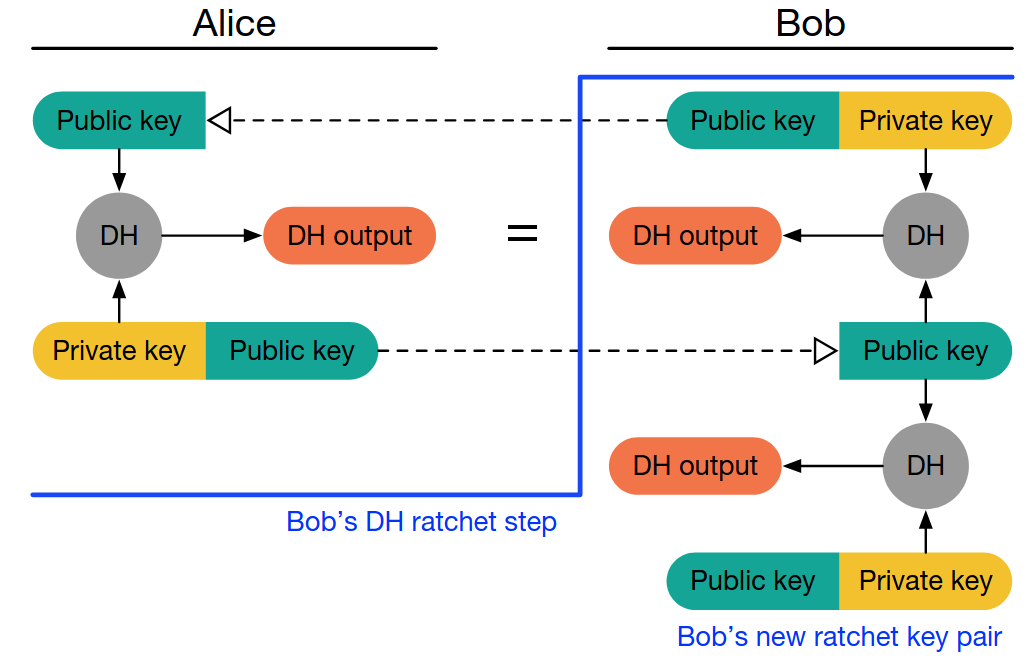
\includegraphics[scale=0.25]{dr2.png}
  \caption{Bob's calculates his DH ratchet step}
  \label{fig:dr2}
\end{figure}

Alice's initial messages advertise her ratchet public key. Once Bob receives one of these messages, Bob performs a DH ratchet step: he calculates the DH output between Alice's ratchet public key and his ratchet private key, which equals Alice's initial DH output. Bob then replaces his ratchet key pair and calculates a new DH output like in figure \ref{fig:dr2}

\newpage

\begin{figure}[ht!]
  \centering
  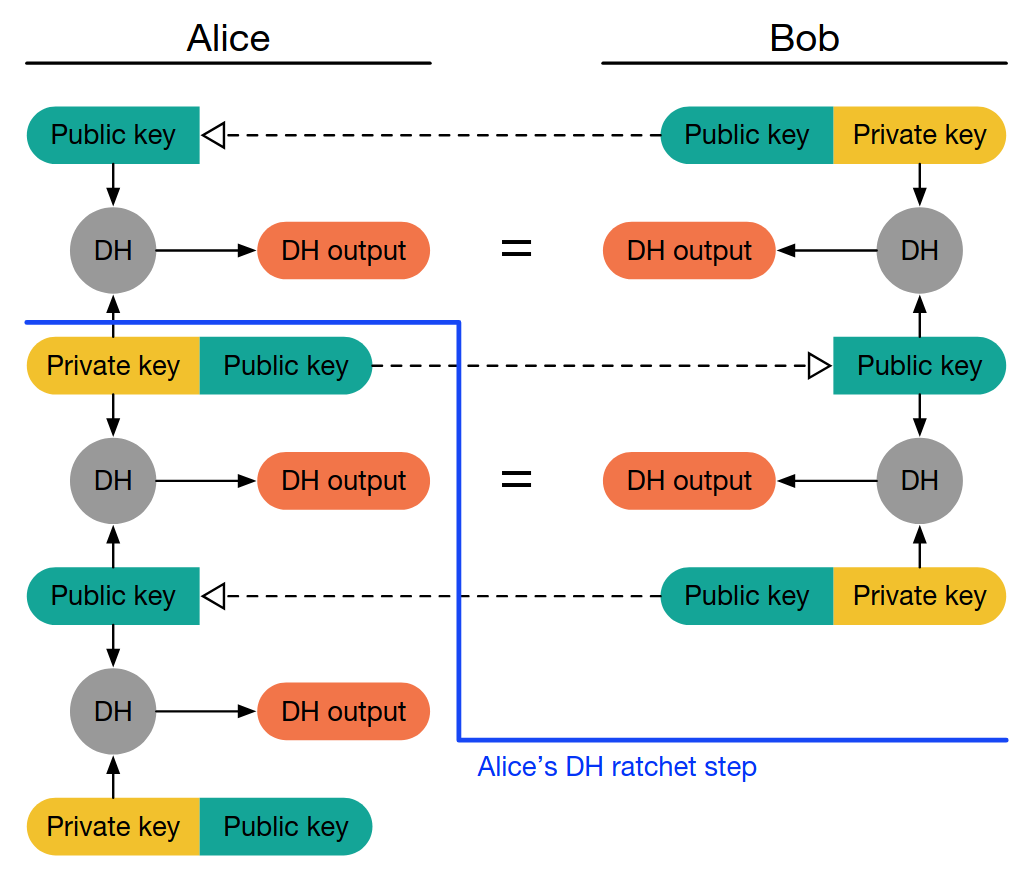
\includegraphics[scale=0.2]{dr3.png}
  \caption{}
  \label{fig:dr3}
\end{figure}

Messages sent by Bob Advertise his new public key. Eventually, Alice will receive one of Bob's messages and perform a DH ratchet step, replacing her ratchet key pair and deriving tow DH outputs, one that matches Bob's latest and a new one \ref{fig:dr3}

\begin{figure}[ht!]
  \centering
  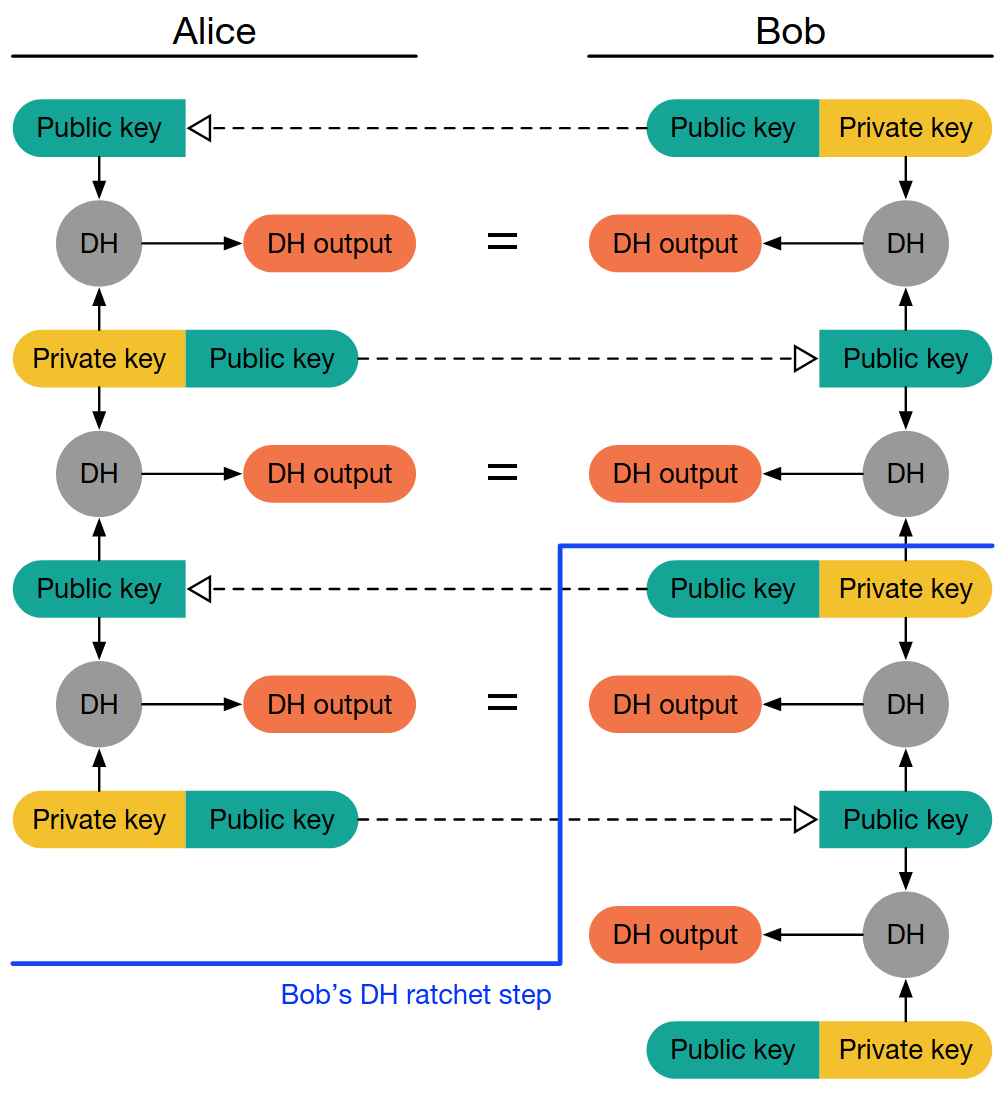
\includegraphics[scale=0.2]{dr4.png}
  \caption{}
  \label{fig:dr4}
\end{figure}

Messages sent by Alice advertise her new public key. Eventually, Bob will receive one of these messages and perform a second DH ratchet step, and so on \ref{fig:dr4}

The DH outputs generated during each DH ratchet step are used to derive new sending and receiving keys. Bob uses his first DH output to derive a receiving chain that matches Alice's sending chain. Bob uses the second DH output to derive a new sending chain. As the parties take turns performing DH ratchet steps, they take turns introducing new sending chains.

However, instead unlike the simplified pictures shown above instead of taking the chain keys directly from DH outputs, the DH outputs are used as KDF inputs to a root chain, and the KDF outputs from the root chain are used as sending and receiving chain keys. Using a KDF chain here improves resilience and break-in recovery. A full DH ratchet step consists of updating the root KDF chain twice, and using the KDF output keys as new receiving and sending chain keys:

\begin{figure}[ht!]
  \centering
  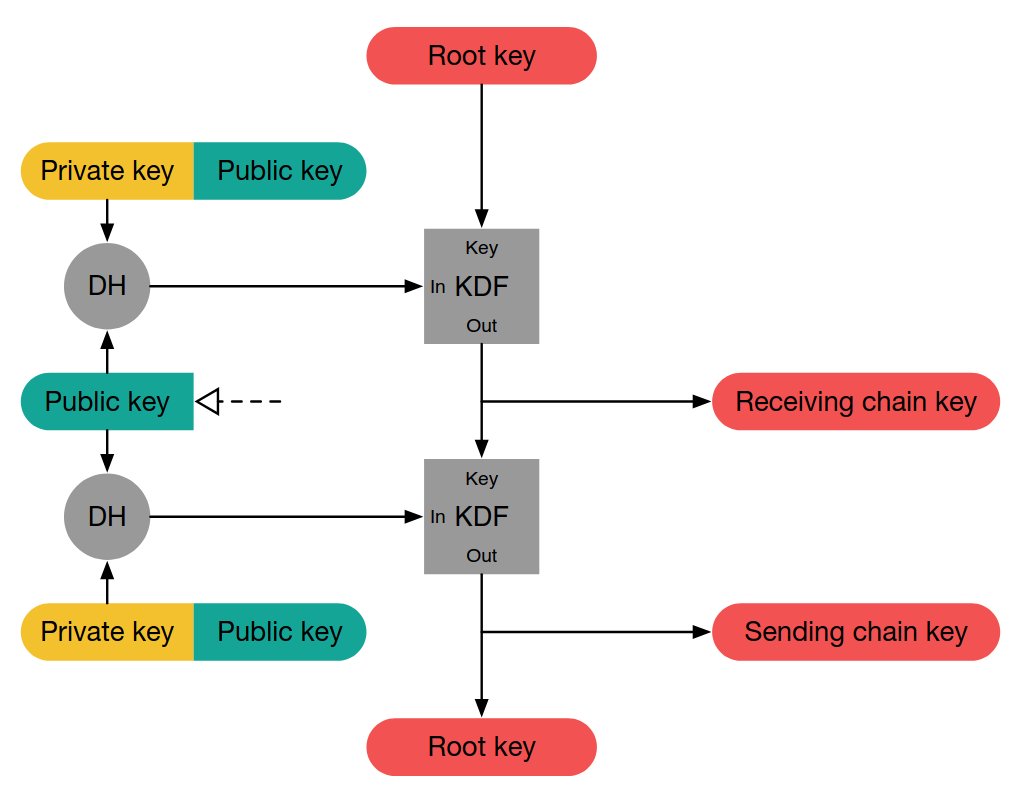
\includegraphics[scale=0.3]{dr5.png}
  \caption{}
  \label{fig:dr5}
\end{figure}

\subsection{Combining both Ratchets}
\label{subsec:CombiningBothRatchets}

Combining the symmetric-key and DH ratchets gives the Double Ratchet:

\begin{itemize}
  \item When a message is sent or received, a symmetric-key ratchet step is applied to the sending or receiving chain to derive the message key.
  \item When a new ratchet public key is received a DH ratchet step is per formed prior to the symmetric-key ratchet to replace the chain keys.
\end{itemize}

In figure \ref{fig:dr6} Alice has been initialized with Bob's ratchet public key and a shared secret which is the initial root key. As part of initialization Alice generates a new ratchet key pair, and feeds the DH output to the root KDF to calculate a new root key $(RK)$ and sending chain key $(CK)$:

\begin{figure}[ht!]
  \centering
  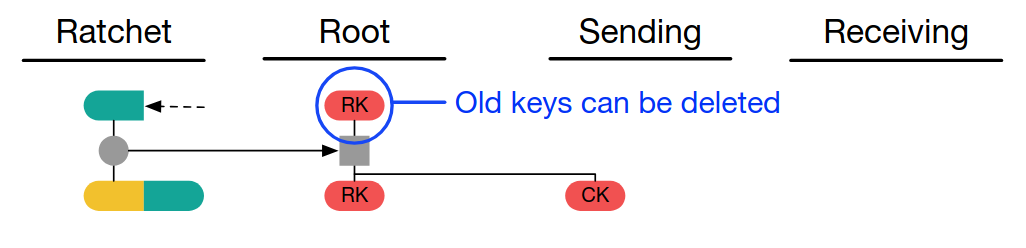
\includegraphics[scale=0.3]{dr6.png}
  \caption{}
  \label{fig:dr6}
\end{figure}

When Alice sends her first message $A1$, she applies a symmetric-key ratchet step to her sending chain key, resulting in a new message key. The new chain key is stored, but the message key and old chain key can be deleted \ref{fig:dr7}

\begin{figure}[ht!]
  \centering
  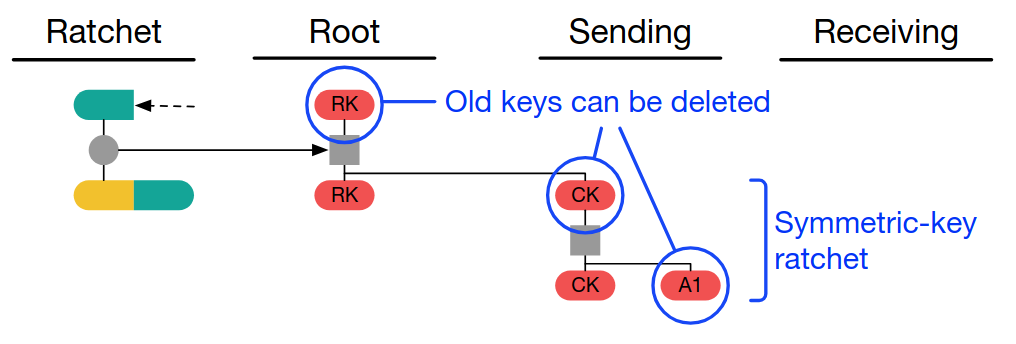
\includegraphics[scale=0.3]{dr7.png}
  \caption{}
  \label{fig:dr7}
\end{figure}

If Alice next receives a response $B1$ from Bob, it will contain a new ratchet public key. Alice applies a DH ratchet step to derive new receiving and sending chain keys. Then she applies a symmetric-key ratchet step to the receiving chain to get the message key for the received message \ref{fig:dr8}

\begin{figure}[ht!]
  \centering
  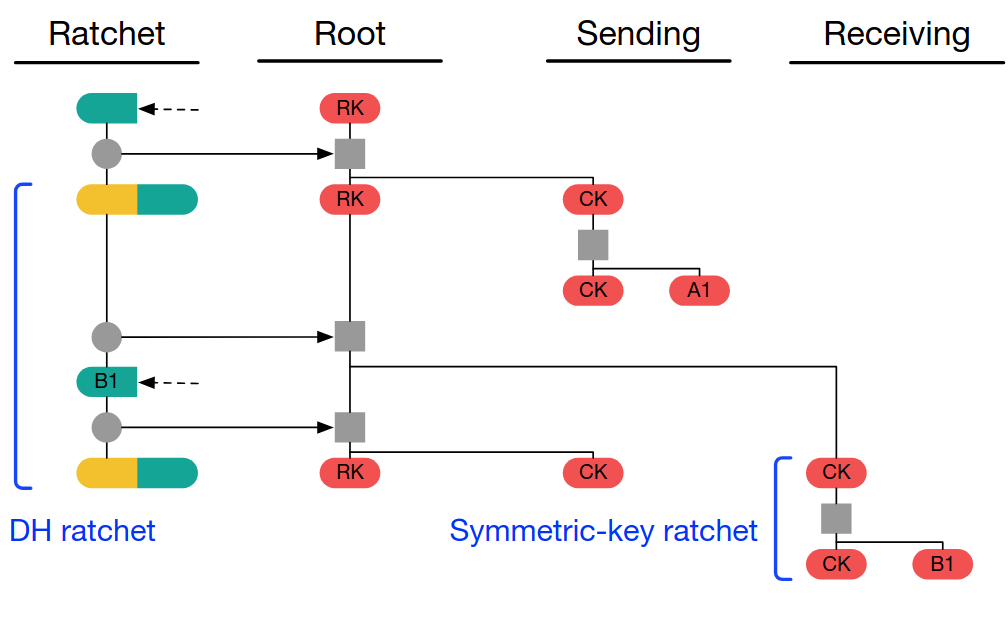
\includegraphics[scale=0.3]{dr8.png}
  \caption{}
  \label{fig:dr8}
\end{figure}

Suppose Alice next sends a message $A2$, receives a message $B2$ with Bob’s old ratchet public key, then sends messages $A3$ and $A4$. Alice’s sending chain will ratchet three steps, and her receiving chain will ratchet once \ref{fig:dr9}

\begin{figure}[ht!]
  \centering
  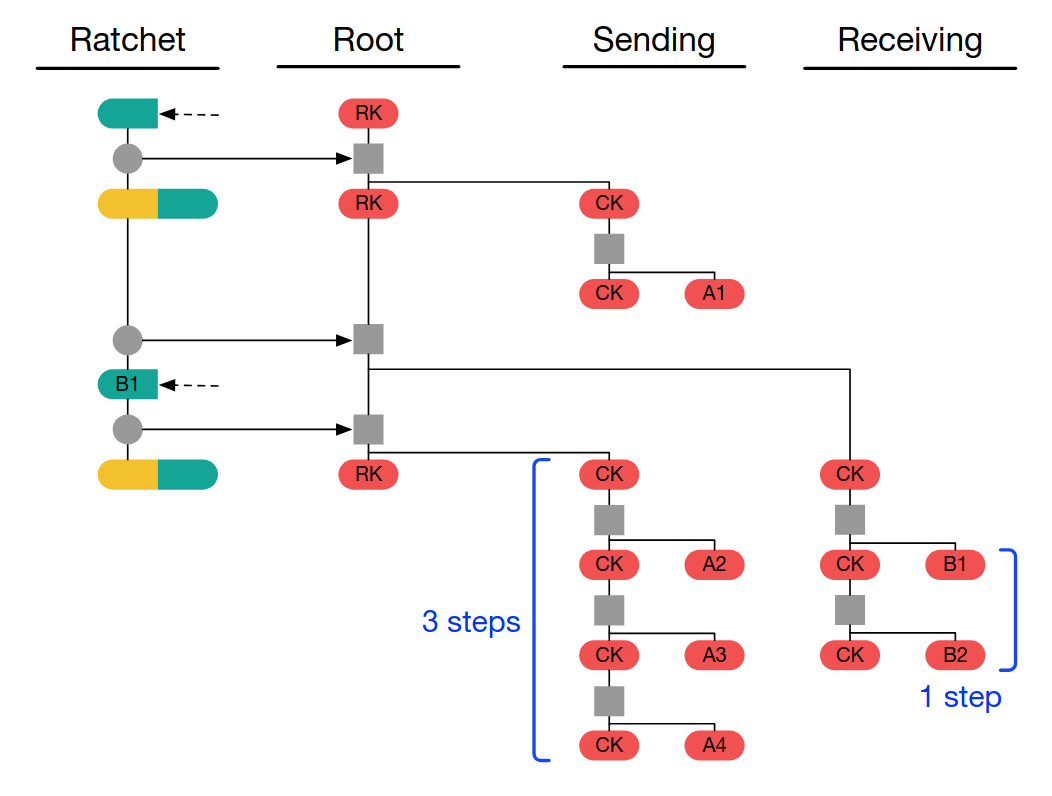
\includegraphics[scale=0.3]{dr9.png}
  \caption{}
  \label{fig:dr9}
\end{figure}

Suppose Alice then receives messages $B3$ and $B4$ with Bob’s next ratchet key, then sends a message $A5$. Alice’s final state will be as follows \ref{fig:dr10}

\begin{figure}[ht!]
  \centering
  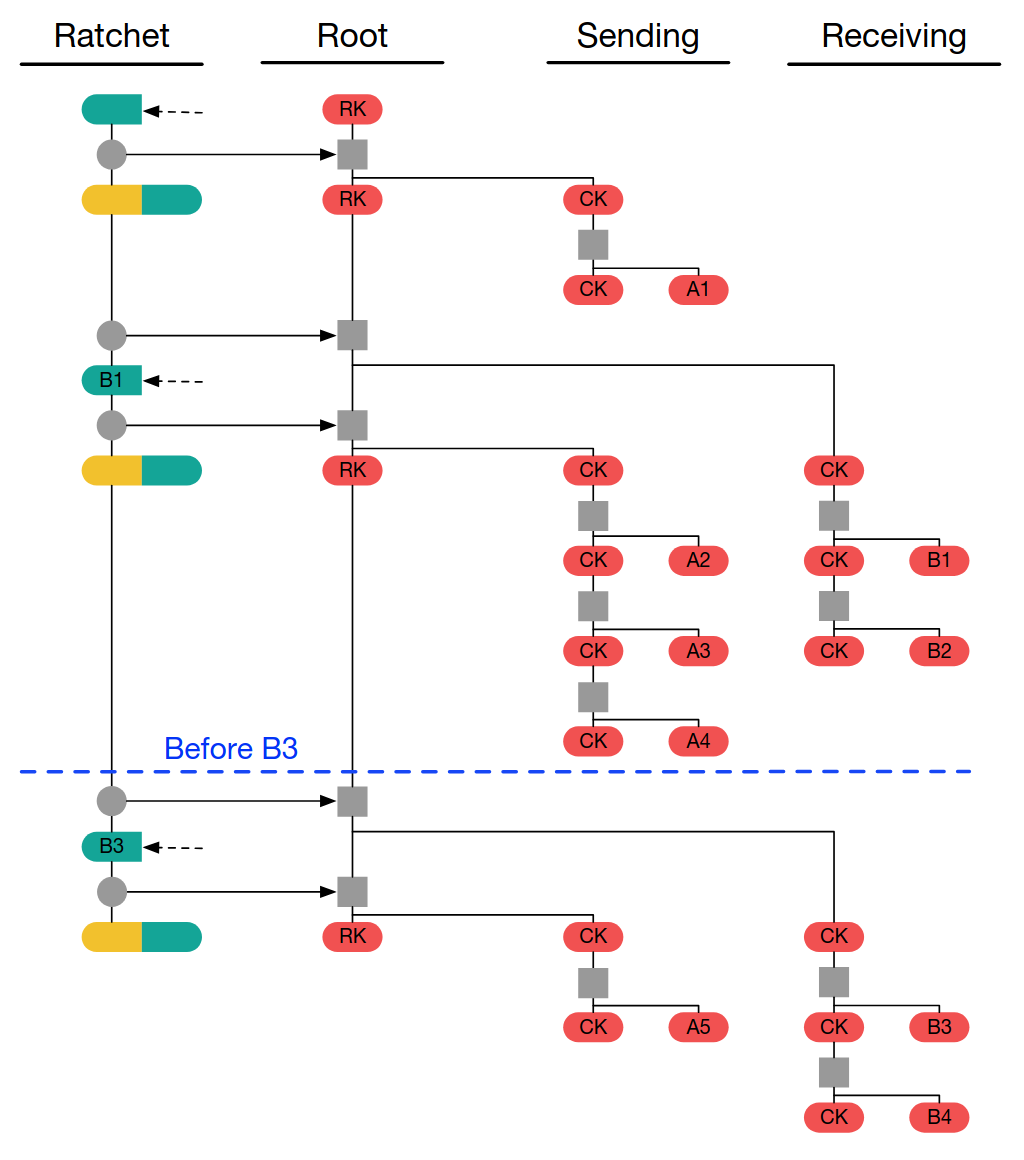
\includegraphics[scale=0.3]{dr10.png}
  \caption{}
  \label{fig:dr10}
\end{figure}

\subsection{Out-of-order messages}
\label{Out-of-orderMessages}

The Double Ratchet handles lost or out-of-order messages by including in each message header the message’s number in the sending chain and the length in the previous sending chain $PN$. This enables the recipient to advance to the relevant message key while storing skipped message keys in case the skipped messages arrive later.

On receiving a message, if a DH ratchet step is triggered then the received $PN$ minus the length of the current receiving chain is the number of skipped messages. The received $N$ is the number of skipped messages in the new receiving chain.

If a DH ratchet step is not triggered, then the received $N$ minus the length of the receiving chain is the number of skipped messages in that chain.

For example, consider the message sequence from the previous section \ref{fig:dr10} when messages $B2$ and $B3$ are skipped. Message $B4$ will trigger Alice’s DH ratchet step (instead of $B3$). Message $B4$ will have $PN = 2$ and $N =1$. On receiving $B4$ Alice will have a receiving chain of length 1 ($B1$), so Alice will store message keys for $B2$ and $B3$, so they can be decrypted if they arrive later as it is shown in figure \ref{fig:dr11}:

\begin{figure}[ht!]
  \centering
  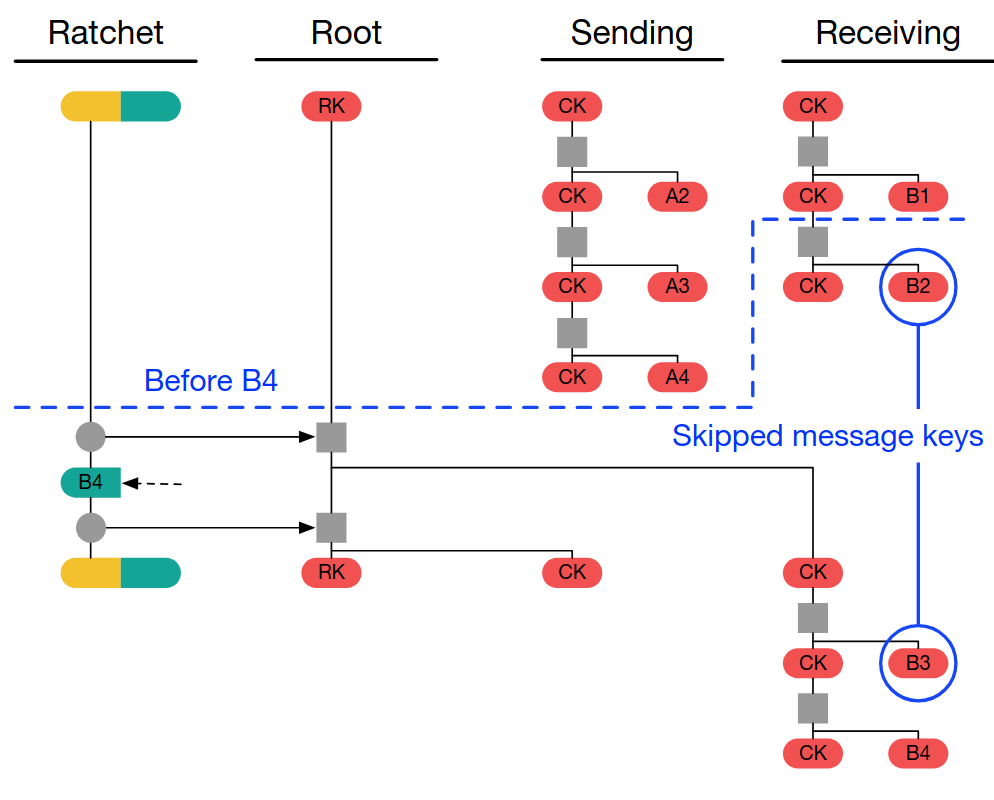
\includegraphics[scale=0.3]{dr11.png}
  \caption{}
  \label{fig:dr11}
\end{figure}

\section{Integration with X3DH}
\label{sec:IntegrationWithX3DH}

The outputs of the X3DH are used by the Double Ratchet:
\begin{itemize}
  \item The $SK$ output from X3DH becomes the $SK$ input to Double ratchet initialization.
  \item The $AD$ output from X3DH becomes the $AD$ input to Double Ratchet encryption and decryption.
  \item Bob's signed prekey form X3DH ($SPK_B$) becomes Bob's initial ratchet public key for double ratchet initialization.
\end{itemize}

\section{Security Considerations}
\label{sec:SecurityConsideration}

\subsection{Authentication}
\label{subsec:Authentication}

Before or after an X3DH key agreement, the parties may compare their identity public keys $IK_A$ and $IK_B$ through some authenticated channel. For example, they may compare public key fingerprints manually, or by scanning a QR code.

During the designing phase of our project we assumed that the server could not be impersonated by any malicious attacker and can not be tampered with thus making sure that what Alice or Bob get from the server are the correct keys.

\subsection{Protocol Replay}
\label{subsec:ProtocolReplay}

One of the potential issues of X3DH is the possibility of a replay attack, but this is no possible thanks to the implementation of the one-time prekys. In Signal's documentation other proposed mitigations are: use a ratchet mechanism, keep a blacklist of observed messages, or replace old signed prekeys more rapidly.

\subsection{Deniability}
\label{subsec:Deniability}

X3DH doesn’t give either Alice or Bob a publishable cryptographic proof of the contents of their communication or the fact that they communicated.

Like in the OTR protocol \cite{OTR}, in some cases a third party that has compromised legitimate private keys from Alice or Bob could be provided a communication transcript that appears to be between Alice and Bob and that can only have been created by some other party that also has access to legitimate private keys from Alice or Bob.

\subsection{Key Compromise}
\label{subsec:KeyCompromise}

Compromise of a party's private keys has a huge impact on security, though the use of ephemeral keys and prekeys provides some mitigation.

Compromise of a party's identity private key allows impersonation of that party to others. Knowledge of a party's preky private keys may affect the security of older or newer $SK$ values, depending on many factors.

Since we implemented one-time prekeys then the compromise of identity keys and preky private keys at some future time will not compromise older $SK$ since the $OPK_B$ was deleted. Moreover, we also implemented double ratchet which replaces $SK$ with new keys to provide fresh forward secrecy.

\subsection{Server Trust}
\label{subsec:ServerTrust}

A malicious server could cause communication between Alice and Bob to fail for example by refusing to deliver messages.

The other possible issue is the inability to check in person keys, but a system similar to the one implemented by many Linux distros should suffice as integrity check for the key of the server. Once we have established a root of trust we can rely on the checks implemented by the protocol.

Another final possible attack is due to the limited number of $OTK$ if an attacker drains another party's one-time prekys, making them unable to create new connections. A system to replenish one-time prekys should be implemented, and the server should limit the rate keys are requested.

\subsection{Secure Deletion}
\label{subsec:SecureDeletion}

The double ratchet algorithm is designed to provide security against and attacker who records encrypted messages and then compromises the sender or receiver at a later time. This security could be deleted if deleted plaintext or keys could be recovered by an attacker with low-level access to the compromised device. But the main focus of this project is security of data in transit.

\subsection{Recovery from Compromise}
\label{subsec:RecoveryFromCompromise}

The DH ratchet is designed to recover security against a passive eavesdropper who observes encrypted messages after compromising the parties to a session. Compromise of secrete keys will:

\begin{itemize}
  \item The attacker could use the compromised keys to impersonate the compromised party.
  \item The attacker could substitute her own ratchet keys via continuous active MitM attack, to maintain eavesdropper on the compromised session.
  \item The attacker could modify a compromised party's RNG so that future ratchet private keys are predictable.
\end{itemize}

If a party suspects its keys or devices have been compromised, it must replace them immediately.

\subsection{Cryptanalysis and Ratchet Public Keys}
\label{subsec:CryptanalysisandRatchetPublicKeys}

Because all DH ratchet computations are mixed into the root key, an attacker who can decrypt a session with passive cryptanalysis, an attacker who can decrypt a session with passive cryptanalysis might lose this ability if she fails to observe some ratchet public keys.

But in our implementation cryptanalysis should not be an issue due to the use of strong encryption function like AES-GCM.

\subsection{Deletion of Skipped Message Keys}
\label{subsec:DeletionofSkippedMessageKeys}

Storing skipped message keys introduces some risks:

\begin{itemize}
  \item A malicious sender could induce recipients to store large numbers of skipped message keys, possibly causing DoS due to consuming storage space.
  \item The lost messages may have been seen by an attacker, even though they did not reach the recipient. The attacker can compromise the intended recipient at a later time to retrieve the skipped message keys.
\end{itemize}

The implemented mitigation is limiting the number of skipped messages to 1000. For the second one we created a set timer after which keys are deleted as proposed by the Signal documentation.


\chapter{Known Limitations}
\label{cha:Limitations}
aaaaaaaaaaaaaaaaaaaa


\chapter{Instruction for Installation and Execution}
\label{cha:Installation}
aaaaaaaaaaaaaaaaaaaa


\printbibliography

\end{document}
